%!TEX root = main.tex

\newpage
\section{Реализация ОА}

Для реализации цифрового автомата использовалась САПР <<Альтера>> Max+plus II.

\subsection{Реализация ОА${}_1$}

Схема построена в соответствии с объединёнными функциями возбуждения и ЛФП, полученными в пункте 3.1.3.

Входными сигналами для ОА${}_1$ являются:
\begin{itemize}
	\item сигнал управления \texttt{Y}, который реализован таким образом, что:
		\begin{itemize}
			\item Y = 1, Y0 = 1. ОА реализует арифметическую операцию, 
			\item Y = 0, Y1 = 1. ОА реализует логическую операцию.
		\end{itemize}
	\item операнд \texttt{B} для логической операции,
	\item сигнал синхронизации \texttt{Q},
	\item сигнал \texttt{LDA} для принудительной установки триггеров в заданное состояние,
	\item сигнал \texttt{SETN} разрешения принудительной установки триггеров в заданное состояние.
\end{itemize}

Выходными сигналами для ОА${}_1$ являются:
\begin{itemize}
	\item новое состояние автомата \texttt{A},
	\item ЛФП \texttt{FS}, \texttt{FZ}, \texttt{FC1}, \texttt{FP}, \texttt{FC}.
\end{itemize}

Поскольку после включения питания все триггеры будут находиться в нулевом состоянии, использована схема принудительной установки состояния автомата в заданное.

Для выполнения различных операций используется одна и та же память, то есть одни и те же триггеры, возбуждаемые различными функциями. Поэтому схемы формирования функций возбуждения и ЛФП представлены в виде отдельных символов oa10\textunderscore logic и oa11\textunderscore logic для ОА$^{(0)}_{1}$ и ОА$^{(1)}_{1}$ соответственно.

Так как используются две схемы формирования функций возбуждения и ЛФП, то реализована схема, позволяющая подключить выходы одной из них к входам триггеров в зависимости от кода операции \texttt{Y}.

\begin{figure}[H]
	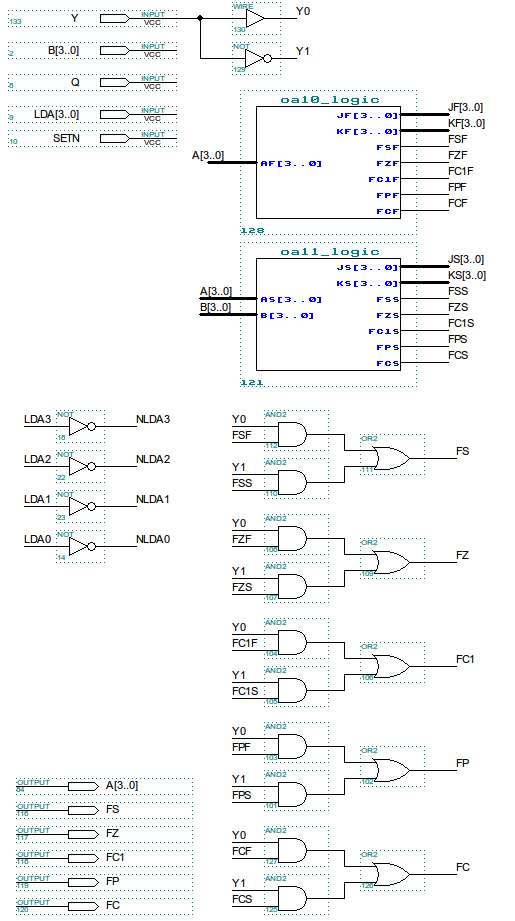
\includegraphics[scale=0.6]{images/altera/rev2/oa1_1_WITH_CONTROL_SIGNAL.png}
	\caption{Cхема ОА$_{1}$ (начало)}
	\label{figure:oa1-1log}
\end{figure}

\begin{figure}[H]
	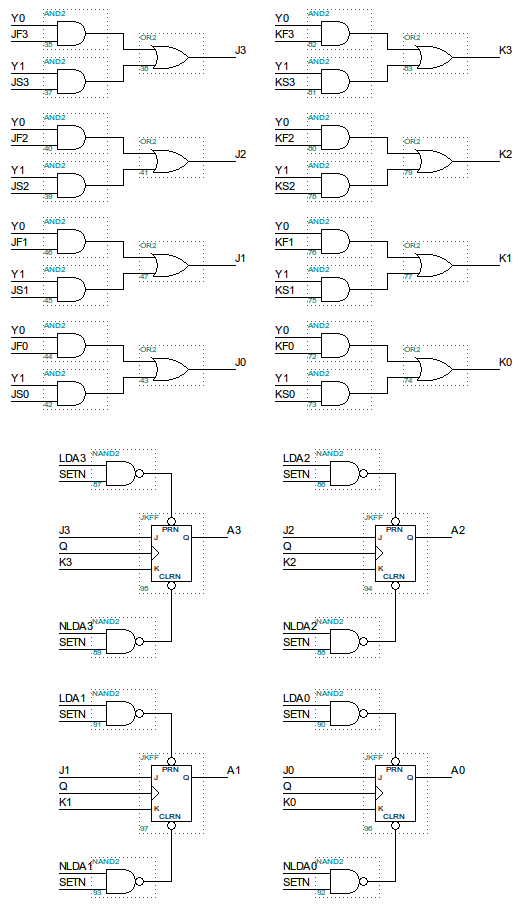
\includegraphics[scale=0.6]{images/altera/rev2/oa1_2.png}
	\caption{Cхема ОА$_{1}$ (окончание)}
	\label{figure:oa1-2log}
\end{figure}

\begin{figure}[H]
	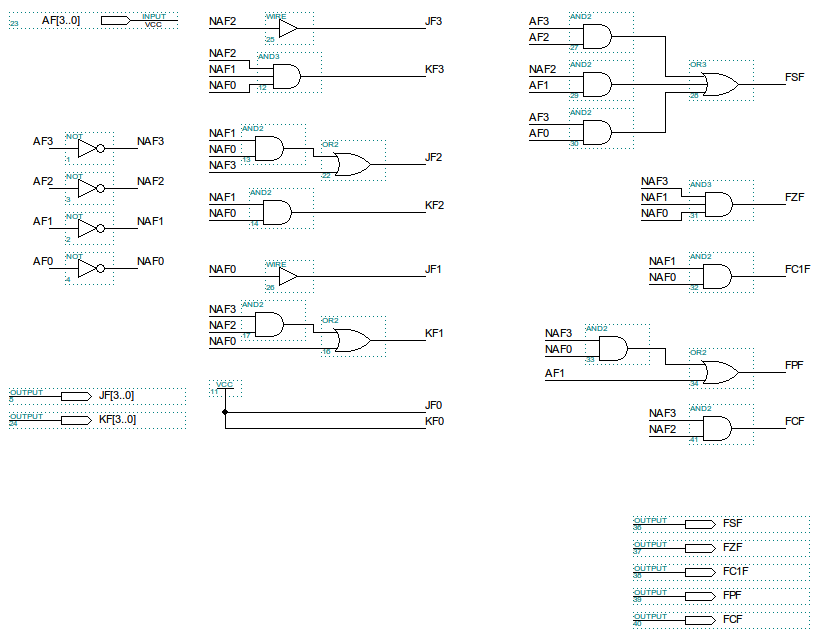
\includegraphics[scale=0.6]{images/altera/rev2/oa10_logic.png}
	\caption{Схема формирования функций возбуждения и ЛФП ОА$^{(0)}_{1}$}
	\label{figure:oa10log}
\end{figure}

\begin{figure}[H]
	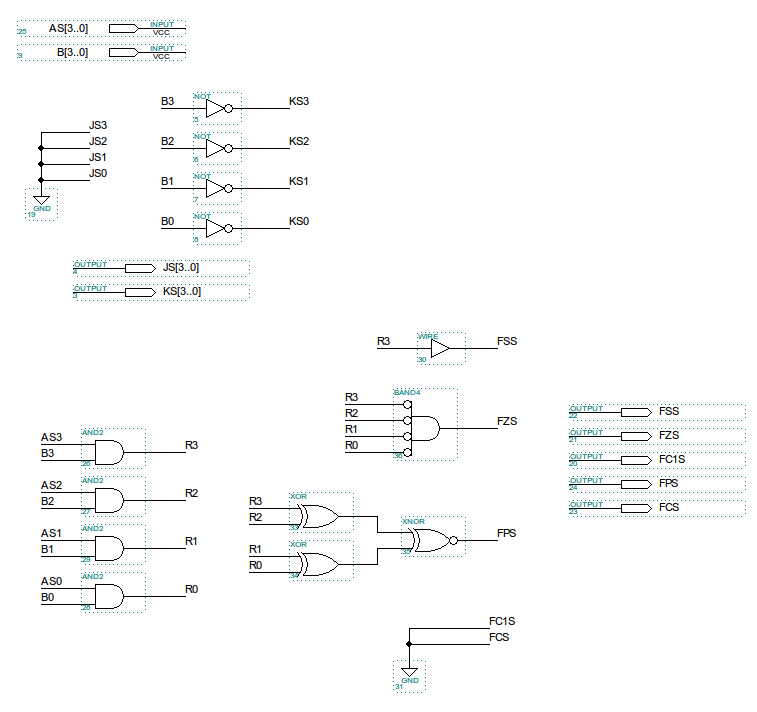
\includegraphics[scale=0.6]{images/altera/rev2/oa11_logic.png}
	\caption{Схема формирования функций возбуждения и ЛФП ОА$^{(1)}_{1}$}
	\label{figure:oa11log}
\end{figure}


\clearpage
\subsection{Реализация ОА${}_2$}

Схема построена в соответствии с объединёнными функциями возбуждения для каждого признака, полученными в пункте 3.2.

Для проверки сохранения значения признака \texttt{C} в соответствии с заданием (Таблица \ref{table:task}) реализован сигнал \texttt{PRNC} принудительной установки признака \texttt{С}. При \texttt{PRNC = 1} автомат устанавливает признак \texttt{C}.

При выполнении логической операции (по сигналу \texttt{Y1}) в соответствии с заданием (Таблица \ref{table:task}) автомат должен устанавливать значения признаков C и C' (на схеме признак С' обозначен как С1) равными нулю. Для этого использован сигнал '0'.

Входными сигналами для ОА${}_2$ являются:
\begin{itemize}
	\item осведомительные сигналы \texttt{FS}, \texttt{FZ}, \texttt{FC1}, \texttt{FP}, \texttt{FC},
	\item сигнал синхронизации \texttt{Q},
	\item сигнал управления \texttt{Y}.
\end{itemize}

Выходными сигналами для ОА${}_2$ являются флаги \texttt{S}, \texttt{Z}, \texttt{C1}, \texttt{P}, \texttt{C}.

\begin{figure}[H]
	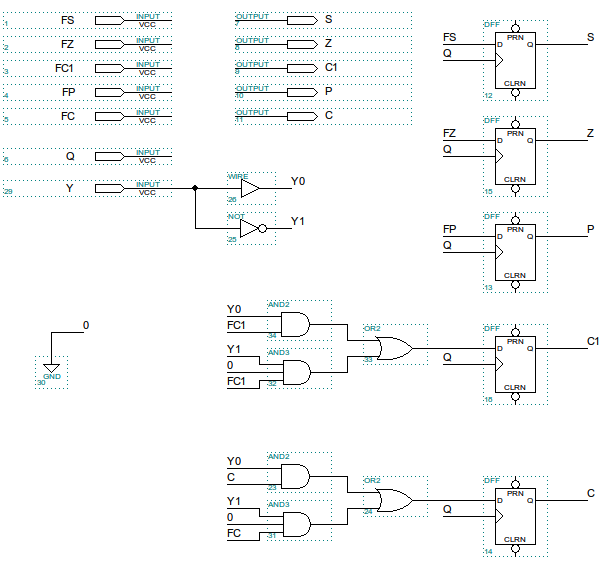
\includegraphics[scale=0.6]{images/altera/rev2/OA2_PRNC/OA2_PRNC_WIDE.png}
	\caption{Cхема ОА$_{2}$}
	\label{figure:oa2log}
\end{figure}

\clearpage
\subsection{Реализация ОА}

Схема операционного автомата (Рисунок \ref{figure:oalog}) представлена в виде совокупности схем ОА${}_1$ и ОА${}_2$, представленных в виде символов.

\begin{figure}[H]
	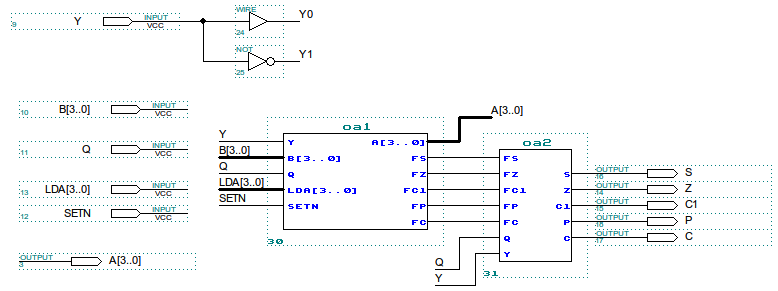
\includegraphics[scale=0.6]{images/altera/rev2/oa_WITH_CONTROL_SIGNAL.png}
	\caption{Cхема ОА}
	\label{figure:oalog}
\end{figure}

\newpage
\section{Моделирование ОА}

\subsection{Методика моделирования}

Процесс моделирования данного автомата был разделен на 3 этапа:
\begin{itemize}
	\item Моделирование ОА$_1$. Целью моделирования ОА1 является проверка правильности выполнении операций, проверка формирования значений логических функций признаков $f_S$, $f_Z$, $f_{C'}$, $f_P$, $f_C$. 
	\item Моделирование ОА$_2$. На данном этапе осуществляется проверка правильности записи значений признаков $S$, $Z$, $C'$, $P$, $C$.
	\item Моделирование ОА. На данном этапе осуществлялась проверка правильности взаимодействия автоматов ОА$_1$ и ОА$_2$. 
\end{itemize}

\subsection{Моделирование ОА$_1$}

\subsubsection{Моделирование арифметической операции}

На вход ОА1 подаются следующие сигналы:
\begin{itemize}
	\item сигнал кода операции \texttt{Y = 1},
	\item сигнал \texttt{LDA = 0011}$_2$, соответствующий числу 3h (первому разрешенному состоянию),
	\item импульс \texttt{SETN}, соответствующий переходу автомата в состояние с шины \texttt{LDA},
	\item импульсы тактовой частоты \texttt{Q}.
\end{itemize}
 
Корректной работе автомата соответствуют значения на выходах, приведенные в таблице \ref{table:oa10test}.

Временная диаграмма результатов моделирования представлена на рисунке \ref{figure:oa10test}.

\clearpage
\begin{table}[H]
	\centering
	\caption{Ожидаемые результаты моделирования операции $A \leftarrow A - 1$}
	\label{table:oa10test}
	\begin{tabular}{|l|*{7}{c|}{r|}} \hline
		A(t) & A(t+1) & FS & FZ & FC1 & FP & FC \\ \hline
		0011 & 1100 & 1 & 0 & 0 & 1 & 1 \\ \hline
		1100 & 1011 & 1 & 0 & 1 & 0 & 0 \\ \hline
		1011 & 1010 & 1 & 0 & 0 & 1 & 0 \\ \hline
		1010 & 1001 & 1 & 0 & 0 & 1 & 0 \\ \hline
		1001 & 1000 & 1 & 0 & 0 & 0 & 0 \\ \hline
  		1000 & 0111 & 0 & 0 & 1 & 0 & 0 \\ \hline
		0111 & 0110 & 0 & 0 & 0 & 1 & 0 \\ \hline
		0110 & 0101 & 0 & 0 & 0 & 1 & 0 \\ \hline
		0101 & 0100 & 0 & 0 & 0 & 0 & 0 \\ \hline
		0100 & 0011 & 0 & 0 & 1 & 1 & 0 \\ \hline
	\end{tabular}
\end{table}

\begin{figure}[H]
	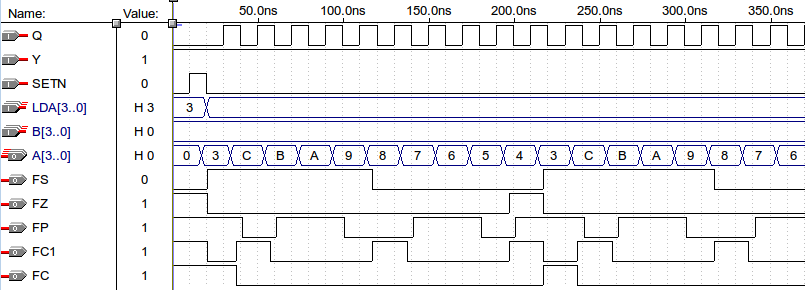
\includegraphics[scale=0.6]{images/altera/rev2/test10.png}
	\caption{Временная диаграмма результатов моделирования операции $A \leftarrow A - 1$}
	\label{figure:oa10test}
\end{figure}

Автомат циклически выполняет заданную операцию $A \leftarrow A - 1$ в коде с избытком 3, вырабатывая сигналы от 3h до Ch в шестнадцатеричной системе счисления. Признаки устанавливаются в соответствии с таблицей \ref{table:oa10test}. То есть автомат функционирует в соответствии с заданием.

\clearpage
\subsubsection{Моделирование логической операции}

На вход ОА1 подаются следующие сигналы:
\begin{itemize}
	\item сигнал кода операции \texttt{Y = 0},
	\item сигналы \texttt{LDA}, соответствующие установке состояния,
	\item импульс \texttt{SETN}, соответствующий переходу автомата в состояние с шины \texttt{LDA},
	\item сигналы \texttt{B},
	\item импульсы тактовой частоты \texttt{Q}.
\end{itemize}
 
Корректной работе автомата соответствуют значения на выходах, приведенные в таблице \ref{table:oa11test}.

Временная диаграмма результатов моделирования представлена на рисунке \ref{figure:oa11test}.

\begin{table}[H]
	\centering
	\caption{Ожидаемые результаты моделирования операции $A \leftarrow A \& B$}
	\label{table:oa11test}
	\begin{tabular}{|l|*{8}{c|}{r|}} \hline
		A(t) & B(t) & A(t+1) & FS & FZ & FC1 & FP & FC \\ \hline
		1010 & 0111 & 0010   & 0  & 0  & 0   & 0   & 0 \\ \hline
		1111 & 1001 & 1001   & 1  & 0  & 0   & 1   & 0 \\ \hline
		1001 & 0110 & 0000   & 0  & 1  & 0   & 1   & 0 \\ \hline
	\end{tabular}
\end{table}

\begin{figure}[H]
	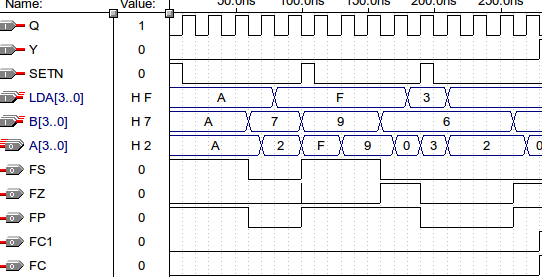
\includegraphics[scale=0.6]{images/ff/11.png}
	\caption{Временная диаграмма результатов моделирования операции $A \leftarrow A \& B$}
	\label{figure:oa11test}
\end{figure}

Из временной диаграммы (Рисунок \ref{figure:oa11test}) видно, что автомат выполняет операцию $A \leftarrow A \& B$ в соответствии с ожидаемыми результатами таблицы \ref{table:oa11test}. 

Если с помощью схемы задания состояния записать в $A$ число 1010$_2$, а на шину $B$ подать сигнал, соответствующий числу 0111$_2$, то после прихода следующего импульса синхронизации $A = A \& B = 1010_2 \& 0111_2 = 0010_2$ и т.д. Признаки устанавливаются в соответствии с таблицей \ref{table:oa11test}. То есть автомат функционирует в соответствии с заданием.

\clearpage
\subsection{Моделирование ОА$_2$}

На триггеры Ds, Dz, Dc1, Dp, Dc подаются:
\begin{itemize}
	\item объединенные функции возбуждения \texttt{FZ}, \texttt{FS}, \texttt{FP}, \texttt{FC1}, \texttt{FC},
	\item управляющий сигнал \texttt{Y},
	\item импульсы тактовой частоты \texttt{Q},
	\item сигнал \texttt{PRNC} принудительной установки признака \texttt{С}.
\end{itemize} 

На выходах ОА$_2$ по положительному фронта синхроимпульса \texttt{Q} записываются значения признаков S, Z, C1, P, C в соответствии со значениями ЛФП из таблиц 2, 5.

\begin{figure}[H]
	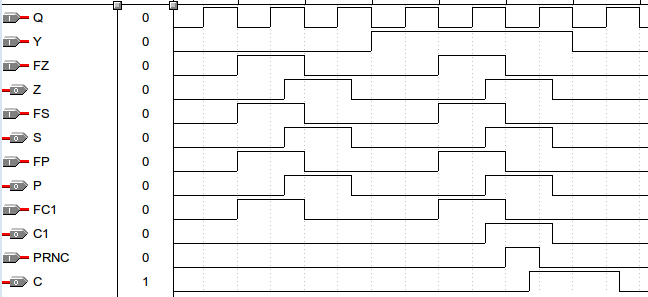
\includegraphics[scale=0.6]{images/ff/2.png}
	\caption{Временная диаграмма результатов моделирования ОА$_2$}
	\label{figure:oa2test}
\end{figure}

Из диаграммы (Рисунок \ref{figure:oa2test}) видно, что схема работает корректно. Значение признака \texttt{C} при выполнении арифметической (Y = 1) операции ОА сохраняет.

\clearpage
\subsection{Моделирование ОА}

На рисунке \ref{figure:oafin0test} приведена временная диаграмма выполнения логической (для Y = 0) и арифметической (для Y = 1) операций, иллюстрирующая работу автомата, состоящего из ОА$_1$ и ОА$_2$.

\begin{figure}[H]
	\begin{subfigure}[b]{1\textwidth}
		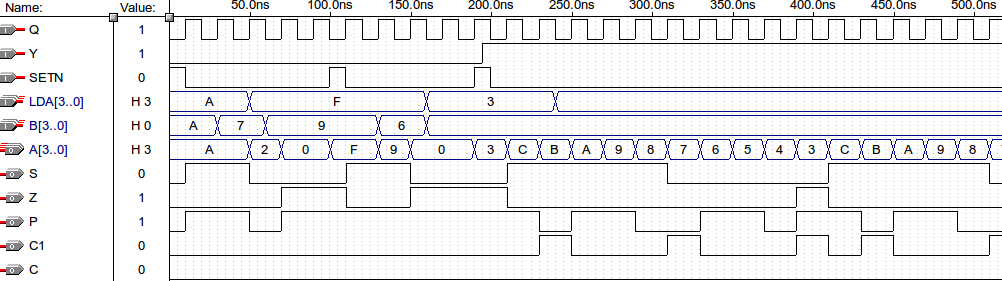
\includegraphics[scale=0.5]{images/ff/001.png}
		\caption{}
	\end{subfigure}
	
	\begin{subfigure}[b]{1\textwidth}
		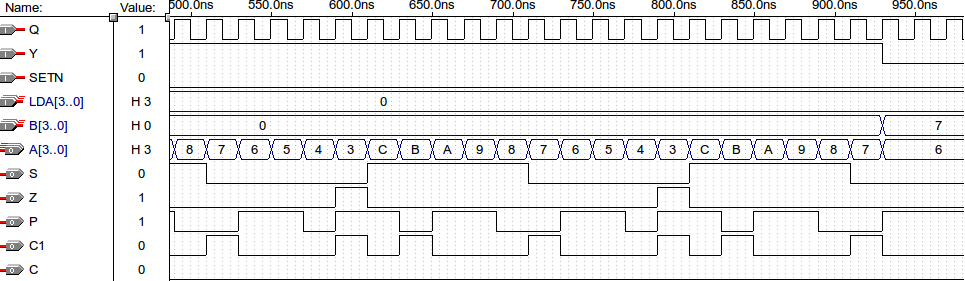
\includegraphics[scale=0.5]{images/ff/002.png}
		\caption{}
	\end{subfigure}
	\caption{Временная диаграмма результатов моделирования ОА}
	\label{figure:oafin0test}
\end{figure}

Из временной диаграммы видно, что результаты выполнения операций и признаки совпадают со значениями из таблиц 2 и 5. Признак \texttt{C}, в соответствии с заданием (Таблица \ref{table:task}), при выполнении арифметической операции ОА не устанавливает.

То есть, автомат функционирует в соответствии с заданием.
